\documentclass[aspectratio=43,11pt]{beamer}

\usetheme{default}
\usecolortheme{default}
\definecolor{aggiemaroon}{RGB}{80,0,0}
\setbeamercolor{structure}{fg=aggiemaroon}
\setbeamertemplate{navigation symbols}{}
\setbeamertemplate{footline}[frame number]
\setbeamertemplate{itemize items}[circle]

\usepackage[utf8]{inputenc}
\usepackage[T1]{fontenc}
\usepackage{graphicx}
\usepackage{amsmath,amssymb}
\usepackage{booktabs}
\usepackage{listings}
\usepackage{tikz}
\usetikzlibrary{arrows.meta,positioning,shapes.geometric,calc,fit}

\graphicspath{{lecture7_alt_figs/}}

\definecolor{cprior}{HTML}{4C78A8}
\definecolor{clik}{HTML}{F58518}
\definecolor{cpost}{HTML}{54A24B}
\definecolor{cgrid}{HTML}{E45756}

% R listings
\lstdefinestyle{rcode}{
  language=R, basicstyle=\ttfamily\scriptsize, keywordstyle=\color{blue!70!black},
  commentstyle=\color{gray!80!black}\itshape, stringstyle=\color{green!40!black},
  backgroundcolor=\color{gray!10}, frame=single, rulecolor=\color{gray!40},
  breaklines=true, showstringspaces=false, columns=fullflexible, keepspaces=true,
  xleftmargin=2pt, xrightmargin=2pt, aboveskip=2pt, belowskip=2pt
}
\lstset{style=rcode}

\tikzset{
  box/.style={draw,rounded corners=2pt,align=center,inner sep=4pt,font=\footnotesize},
  >=Stealth
}

\usepackage{array}
\newcolumntype{L}[1]{>{\raggedright\arraybackslash}p{#1}}
\newcommand{\pic}[2][0.85]{{\centering\includegraphics[width=#1\textwidth]{#2}\par}}

\title{Decision and Risk Analysis}
\subtitle{Lecture 7: \textbf{Approximating the Posterior}\\
{\it Grid Approximation, MCMC, and RStan}\\
(alternative version)
}
\author{}
\date{
\color{aggiemaroon}{
DAEN 427 / ISEN 427 / ISEN 627 - Fall 2026\\
\textbf{Alexander Abuabara}
}
}
\titlegraphic{\vfill 
\includegraphics[height=1.2cm]{TAMU_logo.png}}

\begin{document}

% ---------------------------------------------------------------
\begin{frame}
  \titlepage
\end{frame}

% ---------------------------------------------------------------
\begin{frame}{}
  \begin{enumerate}
    \item \textbf{The problem:} the posterior is often impossible to write down
    \item \textbf{Grid approximation:} brute force, easy to see
    \item \textbf{MCMC:} a smart random walk that scales
    \item \textbf{Diagnostics:} how to know the simulation can be trusted
    \item \textbf{Decisions:} turn posterior draws into risk numbers
  \end{enumerate}
  \vspace{4pt}
  \begin{block}{Example}
    A new component design is tested.\\
    Unknown: its failure probability $\pi$.\\
    Decision: \textbf{keep the design or replace it?}
  \end{block}
\end{frame}

% ---------------------------------------------------------------
\begin{frame}{Why do we need to approximate?}
  \begin{center}
  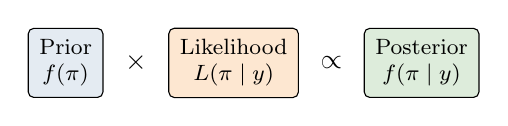
\begin{tikzpicture}
    \node[box,fill=cprior!15] (pr) {Prior\\ $f(\pi)$};
    \node[right=0.15cm of pr] (x1) {$\times$};
    \node[box,fill=clik!20,right=0.15cm of x1] (li) {Likelihood\\ $L(\pi\mid y)$};
    \node[right=0.15cm of li] (x2) {$\propto$};
    \node[box,fill=cpost!20,right=0.15cm of x2] (po) {Posterior\\ $f(\pi\mid y)$};
  \end{tikzpicture}
  \end{center}
  \[
    f(\pi\mid y)=\frac{f(\pi)\,L(\pi\mid y)}{\displaystyle\int f(\pi)\,L(\pi\mid y)\,d\pi}
  \]
  \begin{itemize}
    \item Numerator: easy, we just multiply two functions.
    \item Denominator: an integral, \textbf{hard} for non-conjugate or many-parameter models.
    \item Risk analysis needs numbers such as $P(\pi>\text{threshold}\mid y)$ and expected loss.
    \item We do not need the formula. We need \textbf{a large sample of plausible $\pi$ values} drawn
    from the posterior.
  \end{itemize}
\end{frame}

% ---------------------------------------------------------------
\begin{frame}{Example: component failure probability}
  \begin{columns}[T]
    \begin{column}{0.50\textwidth}
      \small
      \begin{itemize}
        \item Prior from experience: $\pi\sim\text{Beta}(2,8)$\\(typically about 20\%)
        \item Test: $Y=5$ failures\\in $n=10$ units
        \item Model: $Y\mid\pi\sim\text{Bin}(10,\pi)$
        \item Here the answer is known: Beta$(7,13)$.
      \end{itemize}
      \vspace{3pt}
      \textbf{Why start with a solved problem?} So we can \emph{check} the approximations
      against the truth.
    \end{column}
    \begin{column}{0.55\textwidth}
      \pic[1]{f01_prior_lik_post.png}
    \end{column}
  \end{columns}
\end{frame}

% ---------------------------------------------------------------
\begin{frame}{Grid approximation}
  \begin{center}
  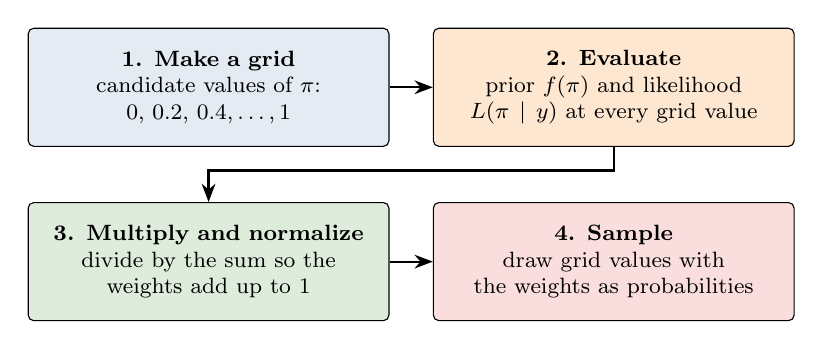
\begin{tikzpicture}[node distance=0.55cm,
      b/.style={box,text width=4.3cm,minimum height=1.5cm}]
    \node[b,fill=cprior!15] (a) {\textbf{1. Make a grid}\\ candidate values of $\pi$:\\ $0,\,0.2,\,0.4,\dots,1$};
    \node[b,fill=clik!20,right=of a] (b) {\textbf{2. Evaluate}\\ prior $f(\pi)$ and likelihood\\ $L(\pi\mid y)$ at every grid value};
    \node[b,fill=cpost!20,below=0.7cm of a] (c) {\textbf{3. Multiply and normalize}\\ divide by the sum so the\\ weights add up to 1};
    \node[b,fill=cgrid!20,right=of c] (d) {\textbf{4. Sample}\\ draw grid values with\\ the weights as probabilities};
    \draw[->,thick] (a)--(b);
    \draw[->,thick] (b.south)--+(0,-0.3)-|(c.north);
    \draw[->,thick] (c)--(d);
  \end{tikzpicture}
  \end{center}
  \small
  Think of it as a \textbf{spreadsheet}: one row per candidate $\pi$, columns for prior,
  likelihood, product, and normalized weight.
\end{frame}

% ---------------------------------------------------------------
\begin{frame}[fragile]{Grid approximation by hand (6 values)}
\begin{lstlisting}
pi_grid      <- seq(from = 0, to = 1, length = 6)       # (1)
prior        <- dbeta(pi_grid, shape1 = 2, shape2 = 8)  # (2)
likelihood   <- dbinom(x = 5, size = 10, prob = pi_grid)
unnormalized <- prior * likelihood                      # (3)
posterior    <- unnormalized / sum(unnormalized)
\end{lstlisting}
  \vspace{-2pt}
  \begin{center}
  \footnotesize
  \begin{tabular}{rrrrr}
    \toprule
    $\pi$ & prior & likelihood & prior$\times$lik. & posterior\\
    \midrule
    0.0 & 0.000 & 0.000 & 0.000 & 0.000\\
    0.2 & 3.020 & 0.026 & 0.080 & \textbf{0.312}\\
    0.4 & 0.806 & 0.201 & 0.162 & \textbf{0.632}\\
    0.6 & 0.071 & 0.201 & 0.014 & 0.056\\
    0.8 & 0.001 & 0.026 & 0.000 & 0.000\\
    1.0 & 0.000 & 0.000 & 0.000 & 0.000\\
    \bottomrule
  \end{tabular}
  \end{center}
  \footnotesize
  \textbf{(1)} grid of candidate $\pi$.\\
  \textbf{(2)} \texttt{dbeta}, \texttt{dbinom} evaluate the
  prior and likelihood at all grid points at once.\\
  \textbf{(3)} Dividing by the sum makes
  the weights a probability distribution.
\end{frame}

% ---------------------------------------------------------------
\begin{frame}{What the 6-point grid looks like}
  \pic[0.95]{f02_grid6.png}
  \footnotesize
  \begin{itemize}
    \item Only $\pi=0.2$ and $0.4$ carry real weight: too coarse to see the shape.
    \item A coarse grid can \textbf{misplace risk}: it has no value between 0.2 and 0.4.
    \item Remedy: a finer grid (next slide).
  \end{itemize}
\end{frame}

% ---------------------------------------------------------------
\begin{frame}[fragile]{Sample from the grid and compare with the truth}
\begin{lstlisting}
grid101 <- grid_post(101)   # same code as before, 101 points
draws <- sample(grid101$pi_grid, size = 10000, replace = TRUE,
                prob = grid101$posterior)           # (4)

ggplot(data.frame(pi = draws), aes(pi)) +
  geom_histogram(aes(y = after_stat(density)), bins = 50) +
  stat_function(fun = dbeta, args = list(shape1 = 7, shape2 = 13))
\end{lstlisting}
  \pic[0.8]{f03_grid_compare.png}
  \footnotesize
  \textbf{(4)} \texttt{sample()} turns weights into a Monte Carlo sample. With 101 points
  the histogram follows the exact Beta$(7,13)$ curve.
\end{frame}

% ---------------------------------------------------------------
\begin{frame}[fragile]{From draws to a risk decision}
\begin{lstlisting}
mean(draws)                       # posterior mean of pi
mean(draws > 0.3)                 # P(pi > 0.3 | data)
quantile(draws, c(0.025, 0.975))  # 95\% credible interval

cost_fail <- 100;  cost_repl <- 30          # cost per unit
c(keep = cost_fail * mean(draws), replace = cost_repl)
\end{lstlisting}
  \pic[0.8]{f04_risk_grid.png}
  \small
  \textbf{Reading it:} $P(\pi>0.3\mid y)\approx 0.65$--$0.67$; expected cost of keeping
  $=100\times0.35=35>30$. Under this loss, \textbf{replace the design}.
\end{frame}

% ---------------------------------------------------------------
\begin{frame}[fragile]{Another model: Gamma--Poisson (failures per month)}
  \small
  Plant has $\lambda$ failures/month. Prior $\lambda\sim\text{Gamma}(3,1)$. Three months of
  data: $y=(2,4,3)$.
\begin{lstlisting}
y        <- c(2, 4, 3)
lam_grid <- seq(0, 12, length = 200)
prior    <- dgamma(lam_grid, shape = 3, rate = 1)
lik      <- sapply(lam_grid,
                   function(l) prod(dpois(y, l)))   # (5)
post     <- prior * lik / sum(prior * lik)
lam_draws <- sample(lam_grid, 10000, replace = TRUE, prob = post)
\end{lstlisting}
  \begin{itemize}
    \item \textbf{(5)} Independent months: the likelihood is a \emph{product} of Poisson probabilities.
    \item Same four steps, different model. The recipe does not change.
  \end{itemize}
\end{frame}

% ---------------------------------------------------------------
\begin{frame}{Gamma--Poisson: grid vs exact}
  \pic[0.78]{f05_gamma_poisson.png}
  \begin{itemize}
    \item Exact posterior: Gamma$(3+9,\,1+3)=$ Gamma$(12,4)$, mean 3 failures/month.
    \item The grid reproduces it. Use it to \textbf{validate} approximations on problems with known answers.
  \end{itemize}
\end{frame}

% ---------------------------------------------------------------
\begin{frame}{The limit of grids: dimensionality}
  \begin{columns}[T]
    \begin{column}{0.52\textwidth}
      \pic[1]{f06_dimension.png}
    \end{column}
    \begin{column}{0.46\textwidth}
      \small
      \begin{itemize}
        \item 100 grid values per parameter.
        \item 1 parameter: 100 points. OK.
        \item 3 parameters: $10^6$ points.
        \item 6 parameters: $10^{12}$ points. Impossible.
      \end{itemize}
      \vspace{4pt}
      Real reliability and risk models often have \textbf{dozens} of parameters.\\[4pt]
      \alert{We need a method that explores only where the posterior is large.}
    \end{column}
  \end{columns}
\end{frame}

% ---------------------------------------------------------------
\begin{frame}{MCMC: the big idea}
  \begin{center}
  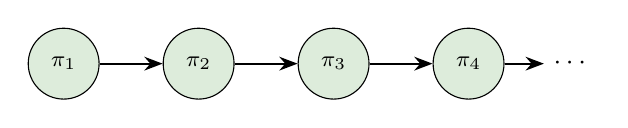
\begin{tikzpicture}[c/.style={circle,draw,fill=cpost!20,minimum size=0.9cm,font=\footnotesize},
                      node distance=0.8cm]
    \node[c] (p1) {$\pi_1$};
    \node[c,right=of p1] (p2) {$\pi_2$};
    \node[c,right=of p2] (p3) {$\pi_3$};
    \node[c,right=of p3] (p4) {$\pi_4$};
    \node[right=0.5cm of p4] (dots) {$\cdots$};
    \draw[->,thick] (p1)--(p2); \draw[->,thick] (p2)--(p3);
    \draw[->,thick] (p3)--(p4); \draw[->,thick] (p4)--(dots);
  \end{tikzpicture}
  \end{center}
  \begin{itemize}
    \item \textbf{Markov chain:} each new value depends \emph{only} on the current one.
    \item The walk is designed so that it \textbf{visits $\pi$ in proportion to posterior density}:
      high-probability regions get many visits, low-probability regions few.
    \item The chain is a list of \emph{dependent} draws, but their histogram approximates the posterior.
  \end{itemize}
  \begin{block}{Analogy}
    An inspector walks a terrain where height = plausibility of $\pi$.
    She mostly stays on high ground, and occasionally steps into valleys.
    Time spent at each location $\approx$ posterior probability.
  \end{block}
\end{frame}

% ---------------------------------------------------------------
\begin{frame}{One Metropolis step}
  \begin{columns}[T]
    \begin{column}{0.6\textwidth}
      \pic[1]{f07_metropolis_step.png}
    \end{column}
    \begin{column}{0.5\textwidth}
      \small
      Only the \textbf{ratio} of heights matters, so the hard denominator cancels!
      \[
        \alpha=\min\left\{1,\frac{f(\pi')L(\pi')}{f(\pi)L(\pi)}\right\}
      \]
      Here:
      \[
        \alpha=\frac{0.087}{0.183}\approx 0.47
      \]
      \begin{itemize}
        \item Uphill proposal: always accepted ($\alpha=1$).
        \item Downhill: accepted with probability $\alpha$.
      \end{itemize}
    \end{column}
  \end{columns}
\end{frame}

% ---------------------------------------------------------------
\begin{frame}{The Metropolis algorithm}
  \begin{center}
  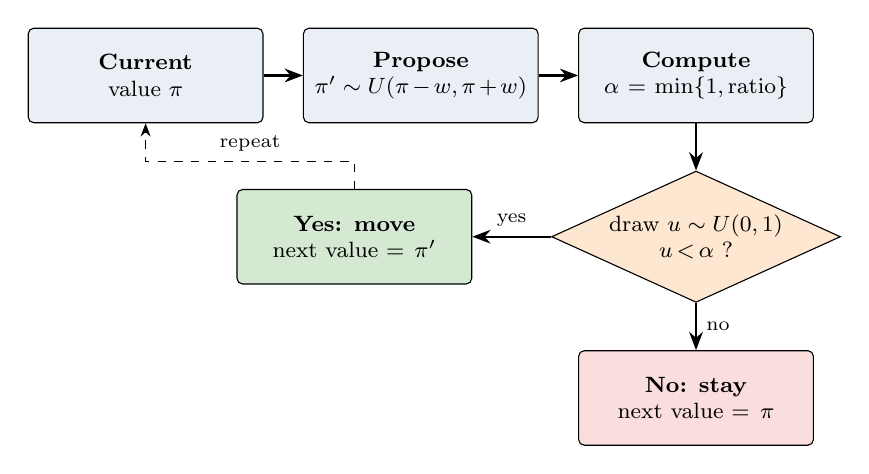
\begin{tikzpicture}[node distance=0.5cm,
      b/.style={box,text width=2.7cm,minimum height=1.2cm,fill=cprior!12}]
    \node[b] (cur) {\textbf{Current}\\ value $\pi$};
    \node[b,right=of cur] (prop) {\textbf{Propose}\\ $\pi'\sim U(\pi-w,\pi+w)$};
    \node[b,right=of prop] (alpha) {\textbf{Compute}\\ $\alpha=\min\{1,\text{ratio}\}$};
    \node[draw,diamond,aspect=2.2,below=0.6cm of alpha,fill=clik!20,font=\footnotesize,inner sep=1pt,align=center] (u) {draw $u\sim U(0,1)$\\ $u\,{<}\,\alpha$ ?};
    \node[b,fill=cpost!25,left=1.0cm of u] (acc) {\textbf{Yes: move}\\ next value $=\pi'$};
    \node[b,fill=cgrid!20,below=0.6cm of u] (rej) {\textbf{No: stay}\\ next value $=\pi$};
    \draw[->,thick] (cur)--(prop); \draw[->,thick] (prop)--(alpha);
    \draw[->,thick] (alpha)--(u);
    \draw[->,thick] (u)--node[above,font=\scriptsize]{yes}(acc);
    \draw[->,thick] (u)--node[right,font=\scriptsize]{no}(rej);
    \draw[->,dashed] (acc.north)--+(0,0.35)-|(cur.south) node[pos=0.25,above,font=\scriptsize]{repeat};
  \end{tikzpicture}
  \end{center}
  \small
  $w$ is the \textbf{step size}. Too small: slow exploration. Too large: many rejections.
\end{frame}

% ---------------------------------------------------------------
\begin{frame}[fragile]{Metropolis in R (and 15 lines)}
\begin{lstlisting}
target <- function(pi) {            # prior x likelihood
  if (pi < 0 || pi > 1) return(0)   # outside (0,1): impossible
  dbeta(pi, 2, 8) * dbinom(5, 10, pi)
}

metropolis <- function(N, w, start) {
  chain <- numeric(N);  current <- start
  for (i in 1:N) {
    proposal <- runif(1, current - w, current + w)       # (a)
    alpha <- min(1, target(proposal) / target(current))  # (b)
    if (runif(1) < alpha) current <- proposal            # (c)
    chain[i] <- current                                  # (d)
  }
  chain
}
chain <- metropolis(N = 5000, w = 0.2, start = 0.5)
\end{lstlisting}
  \small
  \textbf{(a)} propose a nearby value \textbf{(b)} compare heights, the normalizing constant
  cancels \textbf{(c)} accept with probability $\alpha$, else stay \textbf{(d)} record the
  current value, even if we stayed.
\end{frame}

% ---------------------------------------------------------------
\begin{frame}{The chain}
  \pic[0.95]{f08_metropolis_chain.png}
  \begin{itemize}
    \item \textbf{Trace plot:} the chain wanders around 0.35 with no long-term drift.
    \item \textbf{Histogram:} matches the exact Beta$(7,13)$ density (black).
    \item Acceptance rate here: about 66\%.
  \end{itemize}
\end{frame}

% ---------------------------------------------------------------
\begin{frame}[fragile]{In practice: \texttt{rstan}}
  \small You rarely write your own sampler. \textbf{DEFINE} the model, then \textbf{SIMULATE}.
\begin{lstlisting}
library(rstan)
# DEFINE: Stan syntax = data, parameters, model
bb_model <- "
  data { int<lower = 0, upper = 10> Y; }
  parameters { real<lower = 0, upper = 1> pi; }
  model {
    Y  ~ binomial(10, pi);   // likelihood
    pi ~ beta(2, 8);         // prior
  }
"
# SIMULATE: 4 chains, 5000 iterations each (half is warm-up)
bb_sim <- stan(model_code = bb_model, data = list(Y = 5),
               chains = 4, iter = 5000 * 2, seed = 84735)
\end{lstlisting}
  \begin{itemize}
    \item The model block is the \textbf{same math} as before: likelihood and prior.
    \item Warm-up draws are thrown away; \texttt{bb\_sim} keeps $4\times2500=10{,}000$ draws.
  \end{itemize}
\end{frame}

% ---------------------------------------------------------------
\begin{frame}[fragile]{Four chains: first visual check}
\begin{lstlisting}
library(bayesplot)
mcmc_trace(bb_sim, pars = "pi", size = 0.1)    # trace plot
mcmc_dens_overlay(bb_sim, pars = "pi")         # density overlay
\end{lstlisting}
  \pic[0.95]{f09_four_chains.png}
  \small
  Chains start at \emph{different} places, quickly mix into the same band (the
  ``hairy caterpillar''), and give the same density. That is what healthy looks like.
  \par\scriptsize (Figure drawn with the Metropolis sampler; Stan output looks the same.)
\end{frame}

% ---------------------------------------------------------------
\begin{frame}{How do we know the chain is trustworthy?}
  \centering
  \footnotesize
  \begin{tabular}{L{2.5cm}L{3.5cm}L{3.5cm}}
    \toprule
    \textbf{Check} & \textbf{Question} & \textbf{Healthy sign}\\
    \midrule
    Trace plot & Do chains mix and stay stable? & Overlapping ``hairy caterpillars''\\[6pt]
    Density overlay & Do chains agree on the shape? & Curves on top of each other\\[6pt]
    Effective sample size ratio & How many \emph{independent} draws are our draws worth? & $>0.1$\\[6pt]
    Autocorrelation & Does the chain forget the past quickly? & Drops to $\approx 0$ in a few lags\\[6pt]
    $\hat R$ (R-hat) & Do chains agree: between-chain vs within-chain spread & $\approx 1$ ($<1.05$)\\
    \bottomrule
  \end{tabular}
  \begin{alertblock}{}
    {\it A bad simulation is like an uncalibrated sensor: the numbers look plausible but are wrong.
    Always check before you use them.}
  \end{alertblock}
\end{frame}

% ---------------------------------------------------------------
\begin{frame}{Healthy vs unhealthy chains}
  \pic[0.97]{f10_bad_chains.png}
  \begin{itemize}
    \item \textbf{Left:} 4 chains with $w=0.2$ forget their start and overlap.
    \item \textbf{Right:} with $w=0.01$ each chain crawls and is still near its own start:
      the chains disagree. Results would depend on where we began.
  \end{itemize}
\end{frame}

% ---------------------------------------------------------------
\begin{frame}[fragile]{Autocorrelation and effective sample size}
\begin{lstlisting}
mcmc_acf(bb_sim, pars = "pi")      # autocorrelation by lag
neff_ratio(bb_sim, pars = "pi")    # effective size / actual size
\end{lstlisting}
  \pic[0.82]{f11_acf.png}
  \small
  \textbf{Left:} correlation fades after a few lags. \textbf{Right:} neighbours are nearly
  copies of each other. Out of 4500 draws, the healthy chain is worth $\approx 800$
  independent draws, the unhealthy one $\approx 9$.
\end{frame}

% ---------------------------------------------------------------
\begin{frame}[fragile]{R-hat: do the chains agree?}
  \small
  \[
    \hat R\;\approx\;\sqrt{\frac{\text{total variability (within + between chains)}}{\text{typical within-chain variability}}}
  \]
  \vspace{-2pt}
\begin{lstlisting}
rhat(bb_sim, pars = "pi")     # want < 1.05
\end{lstlisting}
  \vspace{2pt}
  \begin{center}
  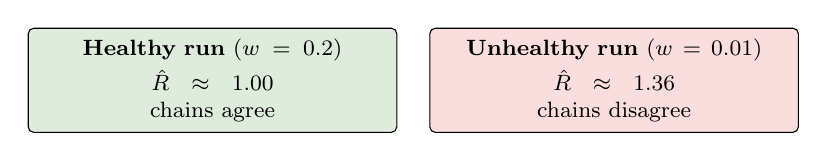
\begin{tikzpicture}
    \node[box,fill=cpost!20,text width=4.4cm] {\textbf{Healthy run} ($w=0.2$)\\[2pt] $\hat R\approx 1.00$\\ chains agree};
    \node[box,fill=cgrid!20,text width=4.4cm] at (5.1,0) {\textbf{Unhealthy run} ($w=0.01$)\\[2pt] $\hat R\approx 1.36$\\ chains disagree};
  \end{tikzpicture}
  \end{center}
  \vspace{2pt}
  \begin{itemize}
    \item If chains explore the same distribution, between-chain spread $\approx$ within-chain spread, so $\hat R\approx1$.
    \item $\hat R$ far above 1: run longer, change the step size or fix the model.
  \end{itemize}
\end{frame}

% ---------------------------------------------------------------
\begin{frame}[fragile]{Use the draws (risk numbers)}
\begin{lstlisting}
pi_draws <- as.data.frame(bb_sim, pars = "pi")$pi
mean(pi_draws)                         # about 0.35
mean(pi_draws > 0.3)                   # about 0.66
quantile(pi_draws, c(0.025, 0.975))    # about (0.16, 0.57)
\end{lstlisting}
  \pic[0.7]{f12_mcmc_decision.png}
  \small
  Every question becomes counting draws. The conclusion matches the exact answer
  ($0.67$; $(0.16,0.57)$): \textbf{replace} if the cost of a failure is high relative to
  replacement.
\end{frame}

% ---------------------------------------------------------------
\begin{frame}{Grid vs MCMC: when to use which}
  \centering
  \footnotesize
  \begin{tabular}{L{2.3cm}L{3.6cm}L{3.8cm}}
    \toprule
     & \textbf{Grid approximation} & \textbf{MCMC}\\
    \midrule
    Idea & Evaluate the posterior on a fixed grid & Random walk that visits $\pi$ in proportion to the posterior\\[4pt]
    Draws & Independent & Dependent (check ESS)\\[4pt]
    Few parameters & Excellent, simple & Works\\[4pt]
    Many parameters & Fails (grid explodes) & Scales\\[4pt]
    Needs diagnostics? & No, just grid fineness & \textbf{Yes}: trace, ESS, $\hat R$\\[4pt]
    Tools & Base R & \texttt{rstan}, \texttt{bayesplot}\\
    \bottomrule
  \end{tabular}
  \begin{block}{}
    {\it Approximate when you must, \textbf{validate} whenever you can, and always finish with a
    decision-relevant number such as $P(\text{risk}>\text{threshold})$.}
  \end{block}
\end{frame}

% ---------------------------------------------------------------
\begin{frame}{Practice problems}
  \small
  \begin{enumerate}
    \item \textbf{Grid:} Repeat the example with prior Beta$(1,1)$ and $Y=2$ failures in $n=20$.
      Use 6, 50 and 500 grid points. How does $P(\pi>0.2\mid y)$ change?
    \item \textbf{Loss:} Change the cost of a failure to 60 and replacement to 30.
      At what posterior mean does the decision flip?
    \item \textbf{Step size:} Run \texttt{metropolis()} with $w=0.001$, $0.05$, $0.5$, $5$.
      Plot the traces and compute the acceptance rate. Which is best?
    \item \textbf{Diagnostics:} Run 4 chains from starts $0.05,0.3,0.6,0.9$ with $w=0.005$.
      What do trace plots and $\hat R$ say? How many iterations fix it?
    \item \textbf{Poisson:} Replace the Beta-Binomial Stan model by a Gamma--Poisson one
      for the monthly failure data and compare with Gamma$(12,4)$.
  \end{enumerate}
\end{frame}

\end{document}